\documentclass{article}
\usepackage{graphicx} % Required for inserting images
\usepackage{geometry}
\usepackage{amsmath}
\usepackage{listings}
\usepackage{hyperref}

\title{Analisis y Diseño de Algoritmos}
\author{Marco Antonio Bastida Flores}
\date{06 Junio 2023}

\geometry{left = 30mm, right = 25mm, top = 30mm, bottom = 20mm}

%------------------------------------------------------------------------%

\begin{document}

\maketitle

En el presente reporte se muestra el desarrollo del algoritmo para obtener el n-esimo numero de Fibonacci utilizando un algoritmo logaritmico.

\section{Fibonacci}

La serie de fibonacci se puede obtener de manera matricial utilizando la siguinete formula:

\vspace{5mm} %5mm vertical space

\begin{displaymath}
    \begin{bmatrix}
        0 & 1 \\
        1 & 1 
    \end{bmatrix}^n
=
    \begin{bmatrix}
        f_n-1 & f_n \\
        f_n & f_n+1 
    \end{bmatrix}
\end{displaymath}

\vspace{5mm} %5mm vertical space

Se puede observar que al multiplicar 
\begin{math}
    \begin{bmatrix}
        0 & 1 \\
        1 & 1 
    \end{bmatrix}
\end{math}
por si misma n veces, se obtiene 
\begin{math}
    f_n
\end{math}
que representa el n-esimo numero de la serie de Fibonacci. Y 
\begin{math}
    f_n+1
\end{math}
que representa el siguiente número en la serie de Fibonacci. \newline
El código para la multiplicación de dos matrices cuadradas se muestra a continuación.

\vspace{5mm} %5mm vertical space

%\begin{lstlisting}[language=Python]
\lstinputlisting[language=Python]{mat_multi.py}
%\end{lstlisting}

\vspace{5mm} %5mm vertical space

Dado que sabemos de antemano que nuestro algoritmo ocupará únicamente matrices cuadradas de 
\begin{math}
    2*2
\end{math}
, podemos hacer uso de las equaciones de Strassen para resolver la multiplicación de una manera sencilla. La función
%\begin{lstlisting}[language=Python]
    mul\_square\_matrix(A, B)
%\end{lstlisting}
Toma dos matrices cuadradas A y B y retorna el resultado de la multiplicación A * B.

\section{Exponenciación}

Para multiplicar n veces la matriz base, utilizaremos el algoritmo de "squaring by exponentiation" que se repesenta de la siguiente manera:

\vspace{5mm} %5mm vertical space

\begin{displaymath}
    x^n = \left\lbrace\begin{array}{c}
    x(x^2)^{(n-1)/2}~~~~~Si~n~es~impar\\
    (x^2)^{n/2}~~~~~~~Si~n~es~par
    \end{array}\right.
\end{displaymath}

\vspace{15mm} %5mm vertical space

El codigo para obtener la potencia de un número usando exponenciación se muestra a continuación:

\vspace{5mm} %5mm vertical space

%\begin{lstlisting}[language=Python]
\lstinputlisting[language=Python]{exponentiation_squared.py}
%\end{lstlisting}

\vspace{5mm} %5mm vertical space

Utilizando las condiciones de la definición se parte el problema por la mitad, utilizando un algoritmo recursivo donde el caso base es cuando el exponente es 0 y el resultado es 1.

\section{Integración de algoritmos para calcular en n-esimo numero de Fibonacci}

Ahora, se integran ambos modulos para obener la n-ésima potencia de la matriz base
\begin{math}
    \begin{bmatrix}
        0 & 1 \\
        1 & 1 
    \end{bmatrix}
\end{math}
para obtener la serie de Fibonacci. \newline
El código se muestra a continuación.

\vspace{5mm} %5mm vertical space

%\begin{lstlisting}[language=Python]
\lstinputlisting[language=Python]{fib_log.py}
%\end{lstlisting}

\vspace{5mm} %5mm vertical space

Se sustituye en el algoritmo de exponenciación la multiplicación de enteros por la multiplicacion de matrices usando la función 
%\begin{lstlisting}[language=Python]
    mul\_square\_matrix(A, B)
%\end{lstlisting}
. El caso base será cuando el exponente n sea igual a 0 y en este caso se hace uso de la matriz identidad
\begin{math}
    \begin{bmatrix}
        1 & 0 \\
        0 & 1 
    \end{bmatrix}
\end{math}
para sustituir el caso base de multiplicar por 1, para ser consistentes con el algoritmo que exponencia numeros enteros y que se toma como base.

\subsection{Resultados}
Para validar que se obtiene la serie de Fibonacci con el algoritmo se hace uso del siguiente snippet:
\vspace{5mm} %5mm vertical space

%\begin{lstlisting}[language=Python]
for n in range(0, 30):\\
        print(n, ": ", fibonacci(n))
%\end{lstlisting}

\vspace{5mm} %5mm vertical space

En la Figura \ref{fig:exponentiation} se puede observar que la secuencia de los números de la serie de Fibonnacci se siguen correctamente.

\vspace{5mm} %5mm vertical space

\begin{figure}[ht]
    \centering
    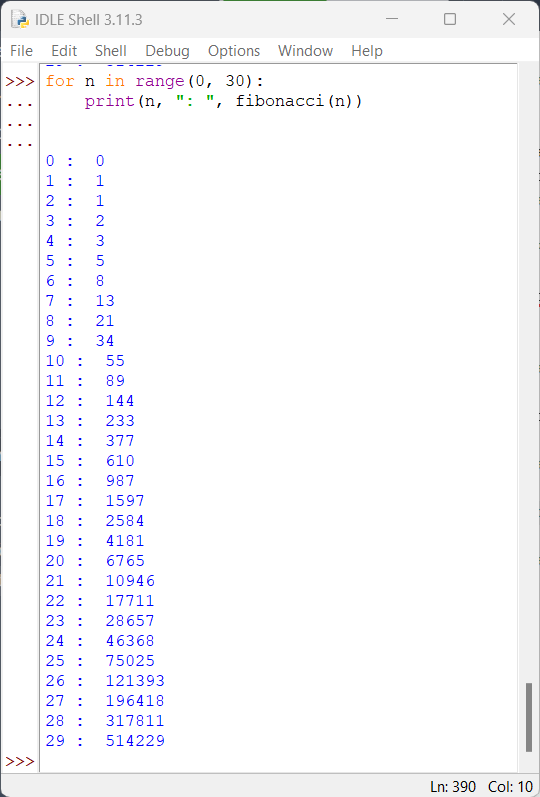
\includegraphics[scale=0.9]{fibonacci_0.png}
    \caption{Validación del algoritmo de potencia por exponenciación}
    \label{fig:exponentiation}
\end{figure}

\vspace{15mm} %5mm vertical space

En la figura \ref{fig:fibo10k} se hace una prueba con un número de Fibonacci igual a 10,000 y se puede observar que el resultado se pinta en consola casi inmediatamente.

\vspace{5mm} %5mm vertical space

\begin{figure}[ht]
    \centering
    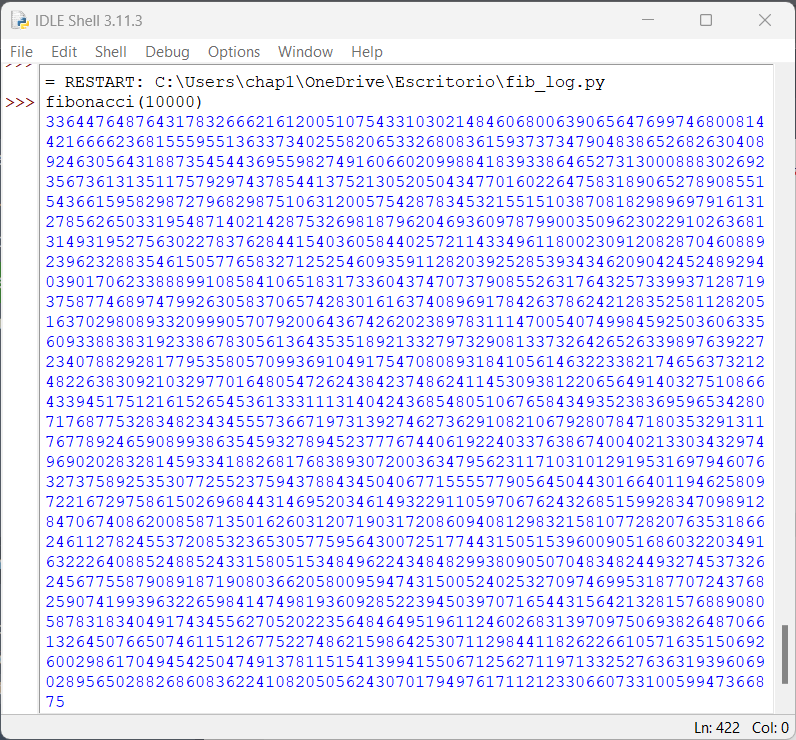
\includegraphics[scale=0.9]{fibonacci_1.png}
    \caption{Algoritmo exponencial para obtener el 10,000 número de Fibonacci}
    \label{fig:fibo10k}
\end{figure}

\vspace{5mm} %5mm vertical space

Por ultimo se muestra en la figura \ref{fig:fibo1M} el calculo de el millonesimo numero de Fibonacci pudiendo observar que el tiempo que tomo para hacer el calculo fue de unos cuantos segundos.

\newpage

\begin{figure}
    \centering
    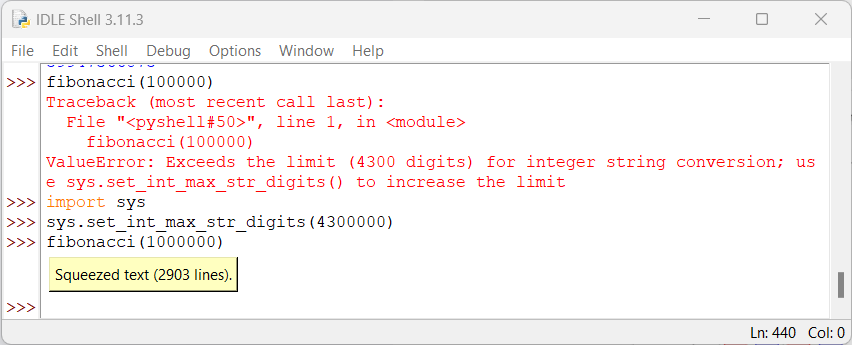
\includegraphics[scale=0.8]{fibonacci_2.png}
    \caption{Algoritmo exponencial para obtener el 1,000,000 número de Fibonacci}
    \label{fig:fibo1M}
\end{figure}

\vspace{15mm} %5mm vertical space

\href{https://github.com/enganthony18/Algorithms}{\includegraphics[scale=0.9]{Git_link.png}}

\end{document}
